\documentclass[a4paper,12pt]{article}
\usepackage{tikz}
\usetikzlibrary{arrows, positioning}
\begin{document}

\title{Reverse Logic via Decision Trees}
\author{Clinton Jon Selke}
\date{\today}
\maketitle

\pagenumbering{roman}
\tableofcontents
\newpage
\pagenumbering{arabic}

\section{Introduction}
The boolean satisfiability problem (SAT) is a problem in logic and computer science which involes assigning true/false values to all variables of a boolean equation such that the entire equation evaluates to true. SAT in general has been proven to be NP-complete. Some of the real world uses of SAT solvers include reverse cryptography, circuit design, artifical integence and automatic theorem proving. In this paper we do something sneaky, we use a sparse truth table data structure and feed it through the circuit structure of the expression, then pull the results out by backtracking from the true/1 leaves of the final sparse truth table back to the root node. We have definitions of the boolean operations AND, OR, and NOT redefined to consume sparse truth table and output sparse truth table. The sparseness in the data structure used for the sparse truth tables opens the door to skiping huge chuncks of the search space, that would otherwise be visited by brute force methods.

Expression $a$ as sparse truth table:

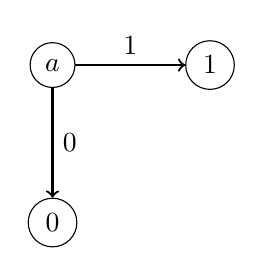
\begin{tikzpicture}[node distance={20mm}, main/.style = {draw, circle},on grid,auto]
	\node[main] (1) {$a$};
	\node[main] (2) [right of=1] {$1$};
	\node[main] (3) [below of=1] {$0$};
	\path[->,draw,thick]
	(1) edge node {$1$} (2)
	(1) edge node {$0$} (3);
\end{tikzpicture}

Expression $\neg a$ as sparse truth table:

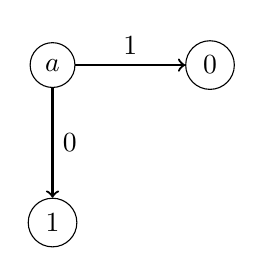
\begin{tikzpicture}[node distance={20mm}, main/.style = {draw, circle},on grid,auto]
	\node[main] (1) {$a$};
	\node[main] (2) [right of=1] {$0$};
	\node[main] (3) [below of=1] {$1$};
	\path[->,draw,thick]
	(1) edge node {$1$} (2)
	(1) edge node {$0$} (3);
\end{tikzpicture}

Expression $a \vee b$ as sparse truth table:

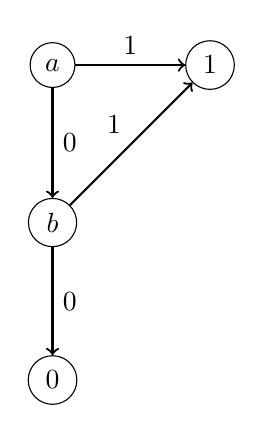
\begin{tikzpicture}[node distance={20mm}, main/.style = {draw, circle},on grid,auto]
	\node[main] (1) {$a$};
	\node[main] (2) [below of=1] {$b$};
	\node[main] (3) [right of=1] {$1$};
	\node[main] (4) [below of=2] {$0$};
	\path[->,draw,thick]
	(1) edge node {$1$} (3)
	(1) edge node {$0$} (2)
	(2) edge node {$1$} (3)
	(2) edge node {$0$} (4);
\end{tikzpicture}

Expression $a \wedge b$ as sparse truth table:

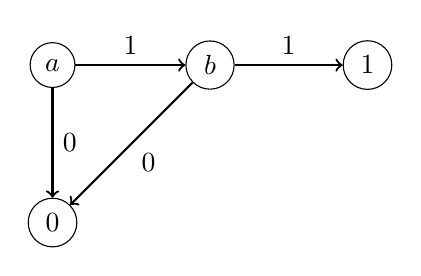
\begin{tikzpicture}[node distance={20mm}, main/.style = {draw, circle},on grid,auto]
	\node[main] (1) {$a$};
	\node[main] (2) [right of=1] {$b$};
	\node[main] (3) [right of=2] {$1$};
	\node[main] (4) [below of=1] {$0$};
	\path[->,draw,thick]
	(1) edge node {$1$} (2)
	(2) edge node {$1$} (3)
	(1) edge node {$0$} (4)
	(2) edge node {$0$} (4);
\end{tikzpicture}

Expression $a \oplus b$ as sparse truth table:

\begin{tikzpicture}[node distance={20mm}, main/.style = {draw, circle},on grid,auto]
	\node[main] (1) {$a$};
	\node[main] (2) [right of=1] {$b$};
	\node[main] (3) [below of=3] {$1$};
	\node[main] (4) [below of=2] {$b$};
	\node[main] (5) [right of=2] {$0$};
	\path[->,draw,thick]
	(1) edge node {$1$} (2)
	(2) edge node {$1$} (5)
	(2) edge node {$0$} (3)
	(1) edge node {$0$} (4)
	(4) edge node {$1$} (3)
	(4) edge node {$0$} (5);
\end{tikzpicture}

\end{document}

